\documentclass[12pt]{exam}

\usepackage[brazil]{babel}
\usepackage{enumerate}
\usepackage[utf8]{inputenc}
\usepackage{graphicx}
\usepackage{usecases}
\extraheadheight{3cm}
\extrafootheight{2cm}
\extrawidth{2cm}
\headrule
\lhead {Universidade Estadual de Campinas 
    \\ Instituto de Computação 
    \\ \bfseries MO620 - Engenharia de Software II - Turma B 
    \\ \textnormal{Aluno: Luiz Alberto Ferreira Gomes}}
\rhead{
    Exercícios do Cap. 1: Introdução 
    \\  RA:007275}
\footrule
\footer{}{Página \thepage\ of \numpages}{}
\renewcommand{\solutiontitle}{\noindent\textbf{Solução:}\enspace}

\printanswers

\begin{document}
  \begin{questions}
    
   
  \question 
    Dado o seguinte enunciado de um sistema de Ponto de Venda (PDV):
    
    Um sistema de ponto de vendas é um sistema computacional usado para registrar vendas e efetuar pagamentos. Ele inclui
    componentes de hardware, como um computador e um \textit{scanner} de código de barras, além dos componentes de software para 
    controle do sistema. Nesse exemplo, estamos interessados na compra e pagamentos de produtos. Os requisitos básicos de 
    funcionamento do sistema são nove: (i) registrar os itens vendidos em cada venda; (ii) calcular automaticamente o total 
    da venda, incluindo taxas; (iii) obter e apresentar as informações sobre cada produto mediante a leitura do seu código de 
    barras; (iv) reportar ao estoque a quantidade de cada produto vendido quando a venda é completada com sucesso; (v) registrar
    cada venda completada com sucesso; (vi) exigir que o atendente forneça sua senha pessoal para que possa operar o sistema; 
    (vii) o sistema deve ter um mecanismo de memória estável;(viii) receber pagamentos em dinheiro ou cartão de crédito, e 
    (ix) emitir mensalmente o balanço de estoque.
    \begin{parts}
      \part Classifique os nove requisitos do sistema de pontos de venda, entre funcionais e não funcionais. Os requisitos
      não-funcionais devem ser categorizados de acordo com a nomenclatura ABNT/ISO 9126.  
      \begin{solution}
	Os requisitos i, ii, iv, v, vi, viii e ix são requisitos funcionais. O requisito iii é um não-funcional de usabilidade e o requisitos vii
	é um não-funcional de confiabilidade.
      \end{solution}
      \part Especifique o diagrama de casos de uso do sistema;
      \begin{solution}
	\begin{center}
	    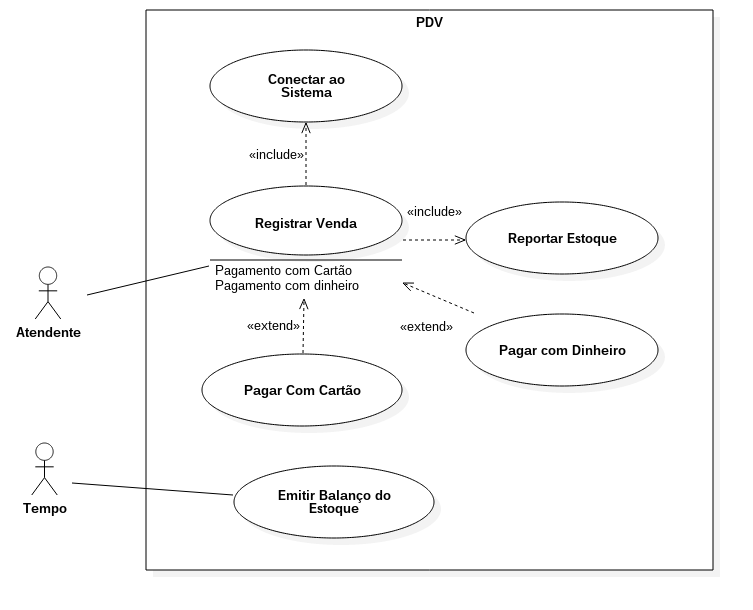
\includegraphics[width=0.5\textwidth]{./exercicios-capitulo2-1b.png}
	\end{center}
      \end{solution}
      
      \part Identifique os relacionamentos entre os diversos casos de uso $<<$include$>>$ e $<<$extend$>>$.
      \begin{solution}
	Identificados no diagrama acima.
      \end{solution}
      \part Descreva um dos casos de uso do sistema usando o formato estudado na disciplina.
      \begin{usecase}
	\addtitle{Caso de Uso}{Registrar Venda}
	\addfield{Ator Primário:}{Cliente}
	\addfield{Ator Secundário:}{Atendente}
	\addfield{Pré-condição:}{O item escolhido está devidamente registrado no estoque.}
	\addfield{Pós-condição:}{
	    \begin{enumerate}
	     \item O item foi vendido ao cliente.
	     \item A venda foi devidamente registrada no sistema.
	     \item O estoque do item foi devidamente atualizado.
	    \end{enumerate}
	  }
	\addscenario{Fluxo Básico:}{
		\item O cliente entra na loja e escolhe os itens que deseja adquirir 
		\item O cliente entrega os itens aos funcionários   	
		\item O funcionário registra cada item no sistema.
		\item O sistema apresenta do total a ser pago
		\item O funcionário mostra o total ao cliente..
		\item O cliente entrega o cartão de crédito ao funcionário.
		\item O funcionário informa ao sistema o número do cartão de crédito.
		8. O sistema autoriza o pagamento
		9. O sistema emite a nota fiscal do cliente.
		10. O funcionário entrega os itens e a nota fiscal ao cliente.
		11. O cliente deixa a loja com os itens escolhidos e com a nota fiscal do itens que comprou.
	}
	\addscenario{Cenários Alternativos:}{
		\item[3.a] O cliente não possui cadastro.
			\begin{enumerate}
			\item[1.] O cliente deverá informar os dados para cadastro.
			\item[2.] O funcionário registra o cadastro.
			\item[3.] O caso de uso retorna ao passo 3 do fluxo principal.
			\end{enumerate}
		\item[3.a] O cliente possui débitos com a locadora
			\begin{enumerate}
			\item[1.] O	cliente paga os seus débitos.		
			\item[2.] O funcionário registra a quitação do débitos.
			\item[3.] O sistema elimina os débitos do cliente.
			\item[4.] O caso de uso retorna ao passo 3 do fluxo principal.
			\end{enumerate}
	}
	\end{usecase}
    \end{parts}
%      \begin{solution}
%        \begin{center}
%	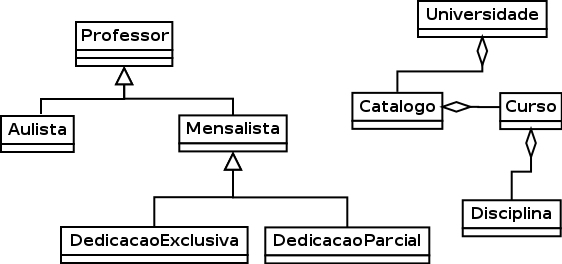
\includegraphics[width=.5\textwidth]{./exercicios-capitulo1-e2.png}
%      \end{center}
%      
%      Enquanto a generalização/especialização é um relacionamento entre classes; a agregação/ decomposição é um relacionamento entre objetos. Ambas promovem o reúso de código, mas de forma diferente. A generalização/especialização por meio da herança e a agregação/decomposição por meio da delegação.
%      
%      
%    \end{solution}
    
    
    
    
    
      
      
        
      
      
  \end{questions}

\end{document}
